\documentclass[../main.tex]{subfiles}
\graphicspath{{./images/}}
%%%%%%%%%%%%%%%%%%%%%%%%%%%%%%%%%%%%%%%%%%%%%%%%%%%%%%%%%%%%%%%%%

\begin{document}


\section{2D approach to object detection} \label{sec:2D_approach}
This section is devoted to a suite of computer vision algorithms that are leveraged to tackle the object recognition task. The array of algorithms tested is as wide as possible, covering both old and new algorithms from the literature.


\subsection{Dataset creation and tooling using a Graphical User Interface} \label{sec:GUI}
Many computer vision algorithms require curated and annotated\footnote{The words annotated and labeled will be used interchangeably.} datasets of images to work. Some are needed to train the algorithm, mainly those that ``learn'' from a subset of the dataset (referred to as \emph{training dataset}) and assess their performance with two other subsets, the \emph{validation} and \emph{testing} datasets. An example of those are Convolutional Neural Networks, or Machine Learning-based algorithm like the Histogram of Oriented Gradients, both explained in this work. Some others are only needed to assess the algorithm's performance, because the features are hardcoded. And some only require a clean database of images to which to compare their input.

Whatever the method used there will always be a need of having quality labeled datasets. There are many methods to do so. Labeling an image that belongs to a certain class can be as simple as storing it inside a folder that has that class' name, or storing the label in plain text in some other file. This tends to be not enough as the goals of the method get harder. For instance, when the bounding box of an object in an image is also required, or a full mask\footnote{``Mask'' in the sense of having some notion of the coordinates of the pixels that belong to a given object. This is also referred to as semantic labeling.} of it. Being such an ubiquitous problem the literature has come up with a varied array of solutions, some more standard than others. As mentioned, some simple classification tasks rely on folder naming to indicate a label class, and in fact most APIs account for that, like OpenCV and TensorFlow, and others vary on the task's difficulty that is being undertaken. 

\paragraph{Labeling style and format}
From all the labeling procedures available the one applied for this thesis has been the most general (and scalable), and that is the labeling style for semantic segmentation. Semantic segmentation is an active area of research in which the every pixel in the input is given a class prediction, similar to the colored mask in figure \ref{fig:gui_labeledimg_mask}. The thing about semantic segmentation and the reason behind its general and scalable labeling style is that it accounts for pretty much all information in the scene by storing the set of pixels that belong to each class. For image classification, the class of the image is the class of the sole mask in the labels file. For object detection with bounding boxes it is the closest-fit rectangle of the set of pixels that belong to each class. In other words, the semantic segmentation style of labeling is the 4x4 of dataset creation. At this point, it has to be noted that none of the algorithms presented in this thesis benefits from having semantic segmentation-styled labels, since no algorithm produces per-pixel classification. Implementing an algorithm that does was an intention at the start of the thesis, but due to time constraints that could not be done. Still, having the most general type of labeling for the dataset is considered as best practice and worth the effort, mainly to its aforementioned scalability.

Having chosen a way in which to perform the labelling, now has to be chosen the specific format. The industry standard regarding semantic segmentation mostly revolves around two formats: the Pascal VOC and the COCO formats. The Pascal Visual Object Classes (VOC) \cite{pascalVOC_2010} is both a dataset and a challenge to develop computer vision algorithms and test them on said dataset, held annually between 2005 and 2012. It has grown over time, and since the 2012th edition includes segmentation labeling. The Common Objects in COntext (COCO) \cite{COCO_paper} is a dataset that was published in 2014 with bounding box and semantic annotations, and has been growing since with new images and features. Despite being both datasets, and not actual labeling formats, they have become so ubiquitous that the labeling style they use has become a standard de facto. The one used in this project is based (although not exactly the same) on the COCO. In my opinion it is easier to understand, and the fact that I have previous experience with it makes it an obvious choice.

\paragraph{Labeling tool}
Having defined the style and format desired for the labeling of the images, tooling is the next logical step. Tooling in the sense of ``what will be used to generate the mentioned labels''. Data curation tends to be the most time-consuming process in a Machine Learning/Deep Learning workflow, so having precise, efficient and productive tools is vital. To that effect, a full-fledged Graphical User Interface (GUI) has been built from the ground up. As mentioned, its main objective is to give the user a quick tool with which to semantically annotate images. The word \emph{quick} can't be stressed enough. Labeling tends to involve thousands of images and many more mouse clicks, making unnecessary actions that could otherwise be avoided is a big time waste in the long-run.

The framework chosen to create the GUI is wxPython, a Python wrapper for wxWidgets. The framework is cross-platform (although it has only been tested in Linux, an Ubuntu distro to be specific) and uses the platform's native API, making it feel like any other app in the OS. Its design is centered around simplicity, always trying to reduce as much as possible avoidable actions from the user to make labeling agile. Figure \ref{fig:gui_labeledimg_annotations} presents the most important elements in the GUI.

Since, as mentioned, the aim is to produce segmentation labels the app includes a canvas in which the user can draw polygons around objects. Every left click creates a new vertex, and a right click unites the last vertex with the first one, hence closing the polygon. See figure \ref{fig:gui_midlabeling_annotations}. If the polygon is deemed to be okay by the user the label can be added. The app manages in the backend the handling of label files: when an image is opened, the app looks in the same directory for a \texttt{.json} file with a filename the same as the image's plus a trailing \emph{\_MASK}\footnote{For instance, image \emph{pepsi\_can.png} would have a corresponding labels file called \emph{pepsi\_can\_MASK.json}.}. If such a file exists, its contents are loaded onto the app so as to inform the user of the actual labels the last time it was edited. If the file doesn't exist, it is created on save. In addition to the aforementioned labeling tools, the GUI also includes two image resizing options (the two buttons at the bottom left of figure \ref{fig:gui_midlabeling_annotations}). Image resizing is very common in computer vision pipelines, either offline or online, since most computer vision algorithms require homogeneously sized inputs. Resizing however comes at a cost: the aspect ratio of the elements of interest (and everything else for that matter) is lost, which could be harmful for the algorithm. This GUI includes an option for standard resizing, where the aspect ratio of the elements is lost, and an option for \emph{seam carving} resizing. Seam carving, also called \emph{content-aware image resizing}, is a rather recent way of reducing or enlarging images without changing the aspect ratio of the meaningful contents inside the image. It computes an energy map of the image with its edges and corners, and then reduces pixels from the seams of pixels that have less energy, thus avoiding much distortion. A full explanation of the seam carving resizing is done in the Appendix \ref{sec:seam_carving}.

\begin{figure}[H]
    \centering
    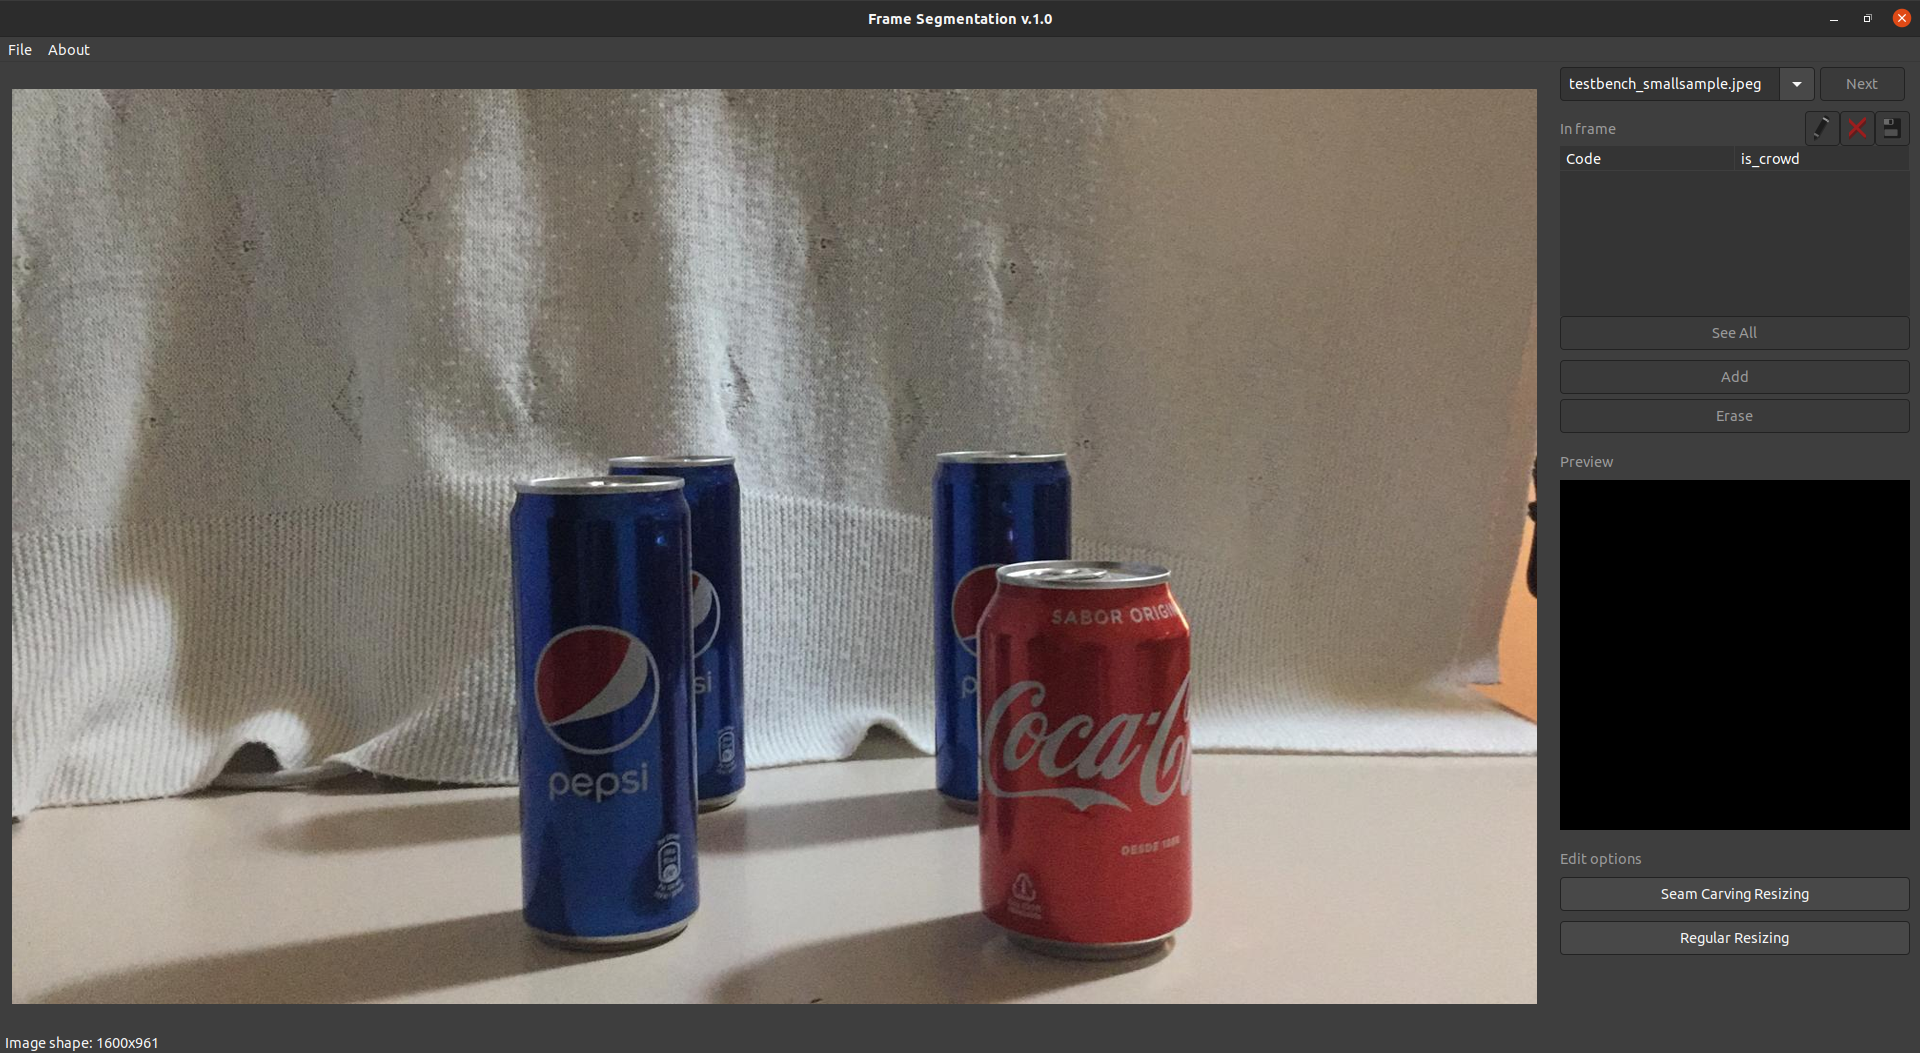
\includegraphics[width=1\linewidth]{images/gui_opening_newimg.png}
    \caption{The Frame Segmentation app when a new unlabeled image is opened. One can tell the image is unlabeled because the list of labels at the right is empty, and none are shown in the preview. The user is also informed by a message in the terminal.}
    \label{fig:gui_opening_newimg}
\end{figure}

\begin{figure}[H]
    \centering
    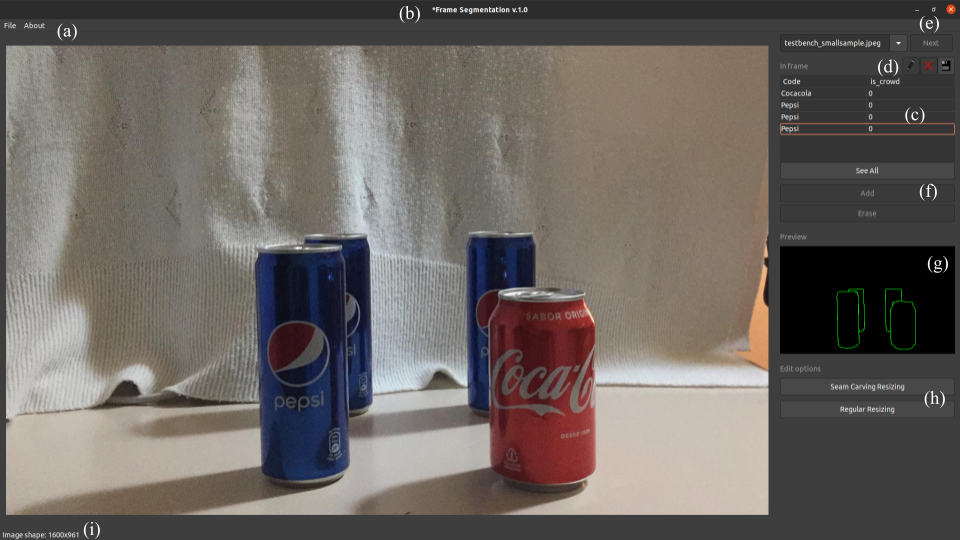
\includegraphics[width=1\linewidth]{images/gui_labeledimg_annotations.png}
    \caption{\emph{(a)}: Customary menubar for any graphical user interface. `File' is a dropdown that is usd to open the image files, and `About' displays some basic information about the app. \emph{(b)}: Name of the opened app along with the version number. The presence of an asterisk at the left indicates that the image has been edited (either because it has been resized or labels have been added or deleted). \emph{(c)}: List of labels present in the image. Double clicking their name will show a colored mask overlaid on top of the element. \emph{(d)}: Main control buttons. The pencil symbol is enabled with a label selected, and allows to change the label name's string. The X button deletes a selected label. The disk symbol saves the listed labels. \emph{(e)}: the app allows to open images one by one or in batches. If more than one image is selected their filename is listed in the dropdown, and the user can cycle through them with the `Next' button. \emph{(f)}: `See All' allows to display all drawn masks at once, overlaid on top of the image, as shown in Figure \ref{fig:gui_labeledimg_mask}. `Add' (enabled after the user has finished a drawing) inserts the drawing into the labels list mentioned in \emph{(c)}. `Erase': discards the drawing done by the user. \emph{(g)}: Preview of the in the labels list mentioned in \emph{(c)}. \emph{(h)}: Two options to resize the present image. The first one uses the \emph{seam carving} algorithm, and the second one standard interpolation. Note: resizing the image will delete existing labels.}
    \label{fig:gui_labeledimg_annotations}
\end{figure}

\begin{figure}[H]
    \centering
    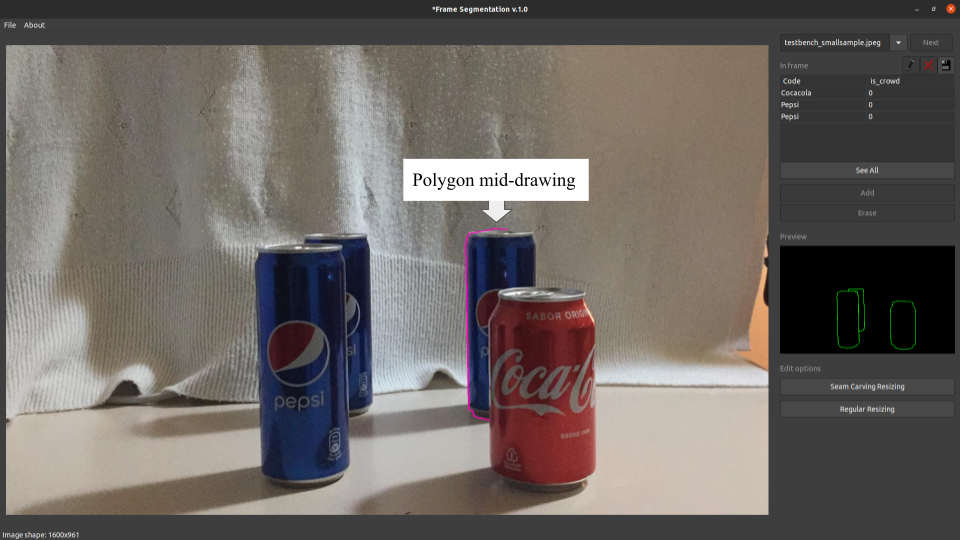
\includegraphics[width=1\linewidth]{images/gui_midlabeling_annotations.png}
    \caption{Screenshot mid labeling. The pink lines are the sides of the polygon created by the user by placing their vertices on the canvas with left clicks. A right click would close the polygon and prompt the user to insert a label name.}
    \label{fig:gui_midlabeling_annotations}
\end{figure}

\begin{figure}[H]
    \centering
    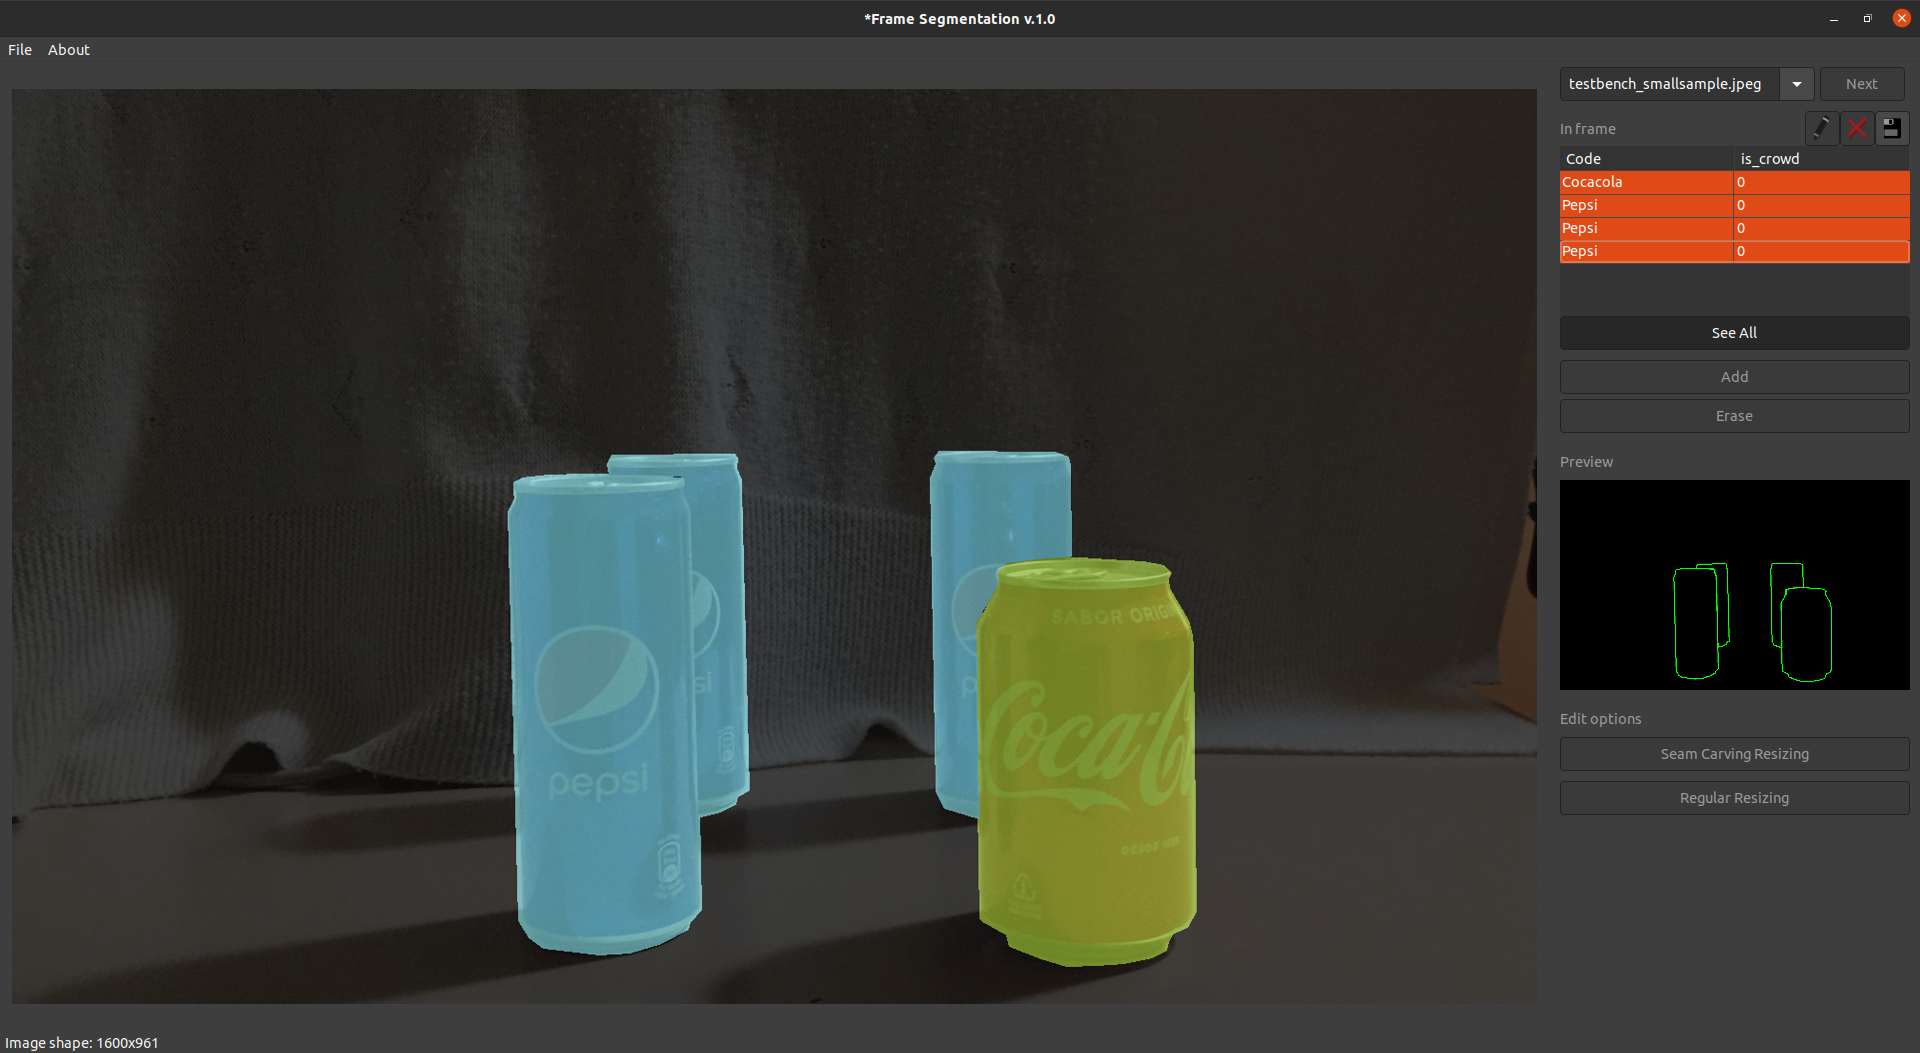
\includegraphics[width=1\linewidth]{images/gui_labeledimg_mask.png}
    \caption{What the user sees when the `See All' button is pressed. The polygons that belong to each label listed at the right are overlaid on top of the image. Colors are chosen randomly every time the button is pressed, but one same label will present the same color for all instances of that label.}
    \label{fig:gui_labeledimg_mask}
\end{figure}

\paragraph{The COCO-styled labels}
As the reader might have noted last paragraphs mention the using of COCO-styled labels by the GUI's backend, but don't mention how. This paragraph aims to shine some light on the matter. The COCO-styled labels contain the following information, in the form of a dictionary:
\begin{itemize}
    \item \texttt{annotation}: a list of arbitrary length, containing
    \begin{itemize}
        \item \texttt{area}: area in the pixels of the segmentation mask.
        \item \texttt{bbox}: area of the bounding that contains the segmentation mask, in the form of $[x_{min}, y_{min}, height, width]$.
        \item \texttt{category\_id}: integer that designates a label.
        \item \texttt{is\_crowd}: When the mask belongs to a collection of objects, rather than a single instance, this is set to 1. For this implementation is left to 0 always.
        \item \texttt{name}: name of the label as a string.
        \item \texttt{segmentation}: this is a list of lists. Each list contains the $x$ and $y$ pixel positions of the vertices of the polygons that make up the mask of a given object (one same object may require more than one polygon if it is occluded by something in the image).
        \item \texttt{supercategory}: Label, as a string, that is semantically higher level (thus encapsulates) than the \texttt{name}. For the current implementation is always left to `None'.
    \end{itemize}
    \item \texttt{info}
    \begin{itemize}
        \item \texttt{contributor}: name of the person or institution to whom belongs the image and label file.
        \item \texttt{description}: description of the image, if necessary.
        \item \texttt{url}: address in the internet from which the image was extracted, if applicable.
        \item \texttt{year}: year in which the labels file is created.
    \end{itemize}
    \item \texttt{image}
    \begin{itemize}
        \item \texttt{file\_name}: file name of the image that corresponds to this label.
        \item \texttt{height}: heigh in pixels of the image.
        \item \texttt{width}: width in pixels of the image.
    \end{itemize}
\end{itemize}

\subsection{The circle Hough Transform}
This section is devoted to the use of an old yet effective method in computer vision literature called the Hough transform, first introduced as a patent in 1962 by Paul Hough \cite{hough1962patent}, and popularized in \cite{ballard1981generalizing_Hough}. This technique, as it will be explained in this section, is used to detect simple shapes of binarized images, where noise and artifacts coming from the binarization may make that task non-trivial. It does so by clustering votes in the parameter space of the model that needs to be identified, be that a line (the model for which it was first designed), circle, ellipse, or any other shape. In this section its powerfulness to detect circular shapes is used, particularly for the Coca-Cola and Pepsi cans, since they present circular-like shapes when seen from the top.

\subsubsection{Theoretical background}
This subsection is devoted to the study of the Hough transform applied to the detection of straight lines, and then moves onto circles.

A line in the Cartesian coordinate system is defined by the equation $y = mx + b$, being $a$ and $b$ the slope and the cut with the y-axis respectively. This same line, however, can also be defined in the polar coordinate system like
\begin{equation}
    y=\left(-\frac{\cos \theta}{\sin \theta}\right) x+\left(\frac{r}{\sin \theta}\right)
\end{equation}
where the radius $r$ and the angle $\theta$ are the parameters that define it. Rearranging the terms, the polar equation is 
\begin{equation} \label{eq:Hough_r}
    r = x \cos \theta + y \sin \theta
\end{equation}

This same line is actually a point in the parameters' $r$ and $\theta$ coordinate spaces. A point in the Cartesian space, however, can be defined by a family of lines that go through it. This family of lines in the parameter space $r$ and $\theta$ of the polar equation is presented in figure \ref{fig:hough_demo_points}. As it can be observed, all lines that may go through a point may take any angle $\theta$ from 0 to 360º with a certain radius $r$ determined by the point's position and angle. To compute it, the input image, in binary form, is iterated pixel per pixel. When a point is detected the corresponding curve in the parameter space is created by testing a number of $\theta$ in \ref{eq:Hough_r} and obtaining the corresponding $r$, also called \emph{distance} in the figure. This creates a set of curves, one per point in the image. Plotted all together, the intersection of the curves are the $r$ and $\theta$ values of a line that goes through the points that created said curves. Repeated intersections are considered peaks. One may establish certain criterions for finding peaks, like thresholds, or a limited number of peaks, to define where to draw the lines in the input image. Figure \ref{fig:hough_demo_points} bottom left takes peaks of 2 or more intersections, while bottom right just takes the highest peak. 

\begin{figure}[htbp]
    \centering
    \resizebox{1\linewidth}{!}{\import{images/}{hough_demo_points.pgf}}
    \caption{\emph{Top left}: binarized input image with consisting of 4 points, 3 of which approximately lined up. \emph{Top right}: the Hough transform obtained from the input image, showing the family of lines that could go through each point. The points where the sinusoidal-shaped curves intersect are the peaks, that is, the values of $r$ and $\theta$ of a line that goes through two or more points. The leftmost peak, which is an intersection of 3 curves, gives the parameters for the downward diagonal line that goes through the three leftmost points in the bottom left image. \emph{Bottom left}: the 4 lines coming from the 4 peaks in the Hough transform. \emph{Bottom right}: The line coming from the highest peak in the Hough transform.}
    \label{fig:hough_demo_points}
\end{figure}

The Hough transform is also robust to some level of noise in the binarized image, as it can be observed in figure \ref{fig:hough_demo_segments_noise}. As one could guess, knowing the amount of lines that need to be found beforehand is very important. If not, one should guess the presence of a line judging the intensity of a peak with respect to the others, and place a threshold somewhere.

\begin{figure}[htbp]
    \centering
    \resizebox{1\linewidth}{!}{\import{images/}{hough_demo_segments_noise.pgf}}
    \caption{\emph{Top left}: 2 segments and noise in the binarized image. \emph{Bottom}: the Hough transform, with the highest peak indicated with an arrow. \emph{Top right}: The line for the $\theta$ and $R$ defined by the highest in the Hough transform, as indicated in the bottom image.}
    \label{fig:hough_demo_segments_noise}
\end{figure}

The Hough transform applied to circles is fundamentally the same. Instead of searching for $r$ and $\theta$ in the parameter space, now one looks for the center coordinates $\left(a, b\right)$, for a given known radius $R$. The peaks in the parameter space will be the aforementioned center coordinates. See figure \ref{fig:hough_demo_circles} for an example. As mentioned before, all pixels in the binary input image are iterated. If the pixel is $True$\footnote{Since, as mentioned, the image is binarized, the data type of the pixels is a boolean.} all circle centers that could have that point as part of its arc are accounted for in the Hough transform, hence creating the circle-like shapes of figure \ref{fig:hough_demo_circles} (bottom), which are all plausible circumference centers. When, in the Hough transform, circumference centers cluster into points this means that there are many pixels in the input image that consider that the point of said cluster could very well be the center of the circumference to which they belong.

\begin{figure}[htbp]
    \centering
    \resizebox{1\linewidth}{!}{\import{images/}{hough_demo_circles.pgf}}
    \caption{\emph{Top left}: input image, binarized. The aim is to find circles with a radius of 20 pixels, of which there are two, one of which intersected by a larger circle. There are lines, noise and an ellipse to make the detection of the circles harder. \emph{Bottom}: the Hough transform for $R=20$. The $x$ axis is the parameter $a$, and the $y$ axis is the parameter $b$. Note that the two peaks can be clearly identified as the points of confluence for the plausible circle centers computed form the points that make up the circumferences in the input image. \emph{Top right}: the two circles of $R=20$ detected in the input image, marked in blue.}
    \label{fig:hough_demo_circles}
\end{figure}

When the radius $R$ is not known, however, the same procedure explained before needs to be repeated for the range of radii that the circles may have. That is, if the circles to be detected have radii in the range $[R_{min}, R_{max}]$, all radii inside this range need to be tested. See figure \ref{fig:hough_demo_all_circles} for an example of this. The input image has circumferences of radii ranging from 15 to 40 pixels, so the entire set of radii $\{15, 16, 17, 18, 19, 20, 21, 22, 23, 24, 25, 26, 27, 28, 29, 30, 31, 32, 33, 34, 35, 36, 37, 38, 39\}$ needs to be tested, hence creating a Hough transform map for each element. To obtain the peaks one needs to compute the most voted points across the set of Hough transforms coming from said set of radii. The 4 peaks found and the radius corresponding to the peaks are shown in the figure, along with the detection of the circles.

\begin{figure}[htbp]
    \centering
    \resizebox{1\linewidth}{!}{\import{images/}{hough_demo_all_circles.pgf}}
    \caption{\emph{Top left}: the input image. the aim is to find the 4 circles of varying radii, disregarding the ellipse and the noise caused by the scattered points and the lines. \emph{Top right}: the successful circle detection. \emph{The 2 rows below}: the Hough transforms coming from the 4 largest peaks in the set of Hough transforms. As it can be observed, the most voted points are the centers of the circumferences of the input image.}
    \label{fig:hough_demo_all_circles}
\end{figure}

\subsubsection{Applying the Hough transform to testbench images from the top}

\subsection{Template matching}

\begin{equation} \label{eq:TM_CCOEFF_NORMED}
    R(x, y)=\frac{\sum_{x^{\prime}, y^{\prime}}\left(T^{\prime}\left(x^{\prime}, y^{\prime}\right) \cdot I^{\prime}\left(x+x^{\prime}, y+y^{\prime}\right)\right)}{\sqrt{\sum_{x^{\prime}, y^{\prime}} T^{\prime}\left(x^{\prime}, y^{\prime}\right)^{2} \cdot \sum_{x^{\prime}, y^{\prime}} I^{\prime}\left(x+x^{\prime}, y+y^{\prime}\right)^{2}}}
\end{equation}

\begin{figure}[htbp]
    \centering
    \resizebox{1\linewidth}{!}{\import{images/}{2pepsi_TM.pgf}}
    \caption{\emph{Left}: identifying the Pepsi cans is easier if the logo is used. \emph{Center}: the inference image for which pyramid and sliding window have been applied, along with the rectangle for the detection. \emph{Right}: the map of similarity values when matching the logo to the inference image. The peak is enclosed by the green circle. Note: since the template matching is applied to all levels of the image pyramid there will be as many matching results as said levels. The figure presented belong to the level with the highest peak (\texttt{maxVal}).}
    \label{fig:2pepsi_TM}
\end{figure}

\begin{figure}[htbp]
    \centering
    \resizebox{1\linewidth}{!}{\import{images/}{0pepsi_testbench_TM.pgf}}
    \caption{The template matching does not work on all instances, however. This figure is a clear example of precisely that.}
    \label{fig:0pepsi_testbench_TM}
\end{figure}

\begin{figure}[htbp]
    \centering
    \resizebox{1\linewidth}{!}{\import{images/}{5milk_testbench2_TM.pgf}}
    \caption{In this example, for instance, the milk brick is perfectly detected. The fact that its front has many edges has indeed helped to avoid confusions with other instances in the scene.}
    \label{fig:5milk_testbench2_TM}
\end{figure}

\subsection{Histogram of Oriented Gradients (HOG) feature descriptor}
The Histogram of Oriented Gradients (HOG) was first introduced by Navneet Dalal and Bill Triggs in \cite{hog_paper} applied to the context of human detection. In their paper they describe it as a global descriptor similar to SIFT \cite{SIFTlowe2004} that, combined with a classifier (they use a Support Vector Machine), can recognize humans in scenes\footnote{Despite centering the paper in human recognition, the authors also mention that the method can work well in other recognition tasks.}. For this thesis, the HOG descriptor is used with an image pyramid and a sliding window over the input image, in combination with a Support Vector Machine and a \emph{k}-Nearest Neighbor classifier to discern between the class labels.

This section is hence divided in three parts: first, the theoretical background behind the Histogram of Oriented Gradients; second, the use of the HOG descriptor with an image pyramid and a sliding window; and third, using the HOG descriptor (which yields an n-dimensional vector) with the \emph{k}-NN and SVM clustering algorithms.

\subsubsection{Theoretical background}
The Histogram of Gradients method is based on the evaluation of local histograms of image gradients and orientations on a grid over the input image, normalized to achieve contrast invariance. The HOG provides a compact and robust enough method to assemble local features (limbs or arms, for instance, in the case of humans) into a single high-dimensional feature vector that can be used with classifiers like \emph{k}-nearest neighbors or Support Vector Machines.

The preliminar step when applying a HOG-based object recognition is to first have a candidate patch in the input image to which apply the descriptor. This may come from an extern method or by a sliding window (both cases are tested in this thesis). Once the image patch is obtained and reshaped to a fixed shape\footnote{Image patches of different shapes yield HOG descriptors of different length, and that must be avoided.} the first step is to compute the gradients in the $x$ and $y$ directions. The Sobel operator \cite{Sobel_operator_history} may be applied, but the authors mention that the difference of pixels works best. To obtain the latter, the kernels $\boldsymbol{k}_{x} = \begin{bmatrix} -1 & 0 & 1 \end{bmatrix}$ and $\boldsymbol{k}_{y} = \begin{bmatrix} -1 & 0 & 1 \end{bmatrix}^{T}$ are convolved to the original image, creating the images $g_{x}$ and $g_{y}$ each. Given the gradients in $x$ and $y$, the magnitude and angle of the gradients at each pixel are computed, with the formulas $g = \sqrt{g_{x}^{2} + g_{y}^{2}}$ and $\theta = \arctan \frac{g_{y}}{g_{x}}$. See figure \ref{fig:pepsi_gradients} for an example of each step of the process. Then, the image patch is divided by cells, which are subsets of pixels. The dimensions of said cells may vary (the authors in \cite{hog_paper} study the performance of using different sizes). For instance, in this work the default cell size of $\left(8x8\right)$ provided by the \emph{Scikit-image} implementation has been used (see figure \ref{fig:pepsi_cellinfo}, where the green grid represents the $\left(8x8\right)$ cells). Then, for each cell, a histogram is computed with the information coming from the magnitude and angle of the gradient at each pixel. The histogram has bins ranging from 0 to 180º, with the bin separation being dependant on the implementation, although the paper uses 9 bins. The bin selection is based on the gradient orientation, and the votes on its magnitude. This vote, however, is proportional to the neighboring bins. In other words, if a gradient has an orientation of 15º and a magnitude of 10, then the 3 quarters of the magnitude will go the bin corresponding to the 20º and only a quarter to the one of 0 º. See the rightmost image in figure \ref{fig:pepsi_cellinfo} for an example. As it can be observed, each cell has its corresponding histogram represented as an arrow.


\begin{figure}[htbp]
    \centering
    \resizebox{1\linewidth}{!}{\import{images/}{pepsi_gradients.pgf}}
    \caption{\emph{From left to right}: (1) the original image (a pepsi can from the testbench). (2) The gradient in the $x$ direction after convolving the kernel $\boldsymbol{k}_{x} = \begin{bmatrix} -1 & 0 & 1 \end{bmatrix}$ to the original image (to the grayscaled image actually). (3) The gradient in the $y$ direction after convolving the kernel $\boldsymbol{k}_{y} = \begin{bmatrix} -1 & 0 & 1 \end{bmatrix}^{T}$ to the original image. (4) The gradient magnitude and (5) its orientation.}
    \label{fig:pepsi_gradients}
\end{figure}

\begin{figure}[htbp]
    \centering
    \resizebox{1\linewidth}{!}{\import{images/}{pepsi_cellinfo.pgf}}
    \caption{\emph{Left}: the original image (a pepsi can from the testbench) with the grid of cells overlaid in green on top. \emph{Center}: the matrices of the gradient magnitude and angle corresponding to the topmost left cell. \emph{Right}: the histogram computed for each cell, represented as an arrow.}
    \label{fig:pepsi_cellinfo}
\end{figure}

Up to this point, a histogram (essentially a feature vector) has been created for each cell in the image patch. To allow for contrast variations this histogram is normalized. Instead of being normalized for the cell in which it was created it is normalized for a larger area, called a \emph{block}. The block's dimensions may vary with the implementation, but \cite{hog_paper} recommends a block of $\left(16x16\right)$ pixels. That is, each block covers 4 cells. The particularity is that the blocks overlap each other since they are slid by steps of $8$ pixels in the $x$ and $y$ directions\footnote{Which means that cells will be slid over 4 times (unless those in edges and corners).}. The authors of the paper mention that there is no issue with that, and in fact enhances performance. The 4 histograms in the cell are concatenated and then normalized with the L2 norm.

The histogram of every block will have a length of $9 \: \text{bins/cell} * 4 \: \text{cells/block} = 36 \: \text{bins/block} $. Concatenating the histogram of all blocks will render a large feature vector, very high dimensional. This feature vector is the one used with the classification algorithm, be it a \emph{k}-NN or SVM.

\subsubsection{HOG applied to the testbench}

\subsection{Scale Invariant Feature Transform (SIFT)}
The Scale Invariant Feature Transform (SIFT) \cite{SIFTlowe2004} algorithm is one of the most influential citations\footnote{62628 citations in Google Scholar at the time of this writing.} in the computer vision literature, particularly in the set of non-learning algorithms. This algorithm, invented and patented by David Lowe in 2004, is still today one of the go-to tools to achieve detection of non-variant rigid form objects. This section will, on the one hand, provide a brief theoretical background of the algorithm (rather than a comprehensive explanation, which wouldn't make sense since the original paper is very clear) and then presents the results of applying it to the testbench.

\subsubsection{Theoretical background}
The SIFT is a method that extracts features that can used for matching between images. Said features are invariant to scale and rotation, and are robust to affine distortion, viewport change, noise and illumination change. The assemble of features may be used for object detection if the matching is performed to a database of images. Said matching identifies clusters of features with the Hough transform to assert they belong to the same object, and verifies it computing the object's pose parameters.

On the one hand, there's the process of generating sets of image features and on the other, the matching of said features to a database. The process of generating sets of features is made of 4 steps: \emph{scale-space extrema detection}, \emph{keypoint localization}, \emph{orientation assignment} and the \emph{keypoint descriptor} itself.

\paragraph{Detection of scale-space extrema}
Candidate keypoints are to be located at positions and scales that are repeatable under different views of one same object. According to \cite{SIFTlowe2004}, locations invariant to scale can be found by looking for stable features across all possible scales. The scale function chosen is $L(x,y,\sigma)$, obtained from convoluting the variable-scale Gaussian function $G(x,y,\sigma)$ with the image $I(x,y)$, like:

\begin{equation}
    L(x, y, \sigma)=G(x, y, \sigma) * I(x, y)
\end{equation}
where
\begin{equation}
    G(x, y, \sigma)=\frac{1}{2 \pi \sigma^{2}} e^{-\left(x^{2}+y^{2}\right) / 2 \sigma^{2}}
\end{equation}
despite using the scale space $L(x,y,\sigma)$ as a function, to detect stable keypoint locations scale-space extrema in the difference of Gaussian function is used, as proposed by the same author in \cite{Lowe1999}. The difference of gaussian $D(x,y,\sigma)$ is computed by the difference of nearby scales

\begin{equation}
    \begin{aligned}
    D(x, y, \sigma) &=(G(x, y, k \sigma)-G(x, y, \sigma)) * I(x, y) \\
    &=L(x, y, k \sigma)-L(x, y, \sigma)
    \end{aligned}
\end{equation}
where $k$ is a multiplicative factor. See figure \ref{fig:scale_space_SIFT} for an example of this.
\begin{figure}[htbp]
    \centering
    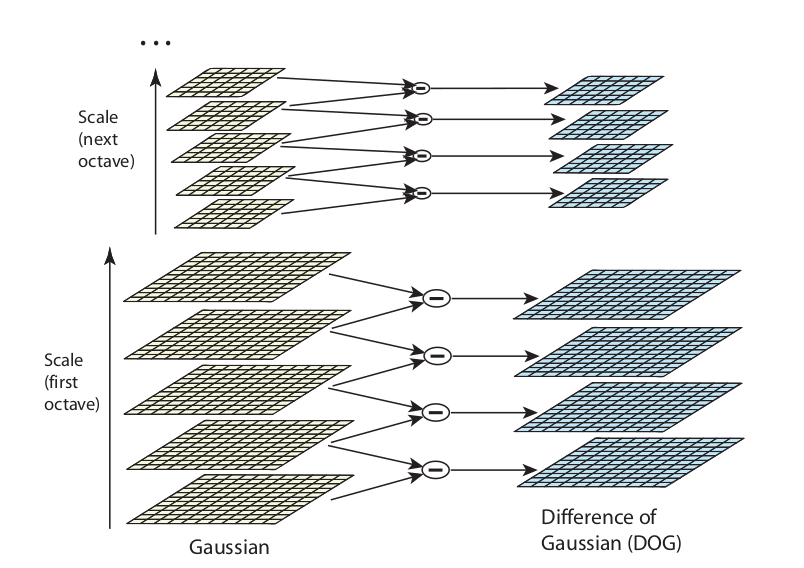
\includegraphics[width=0.9\linewidth]{images/scale_space_SIFT.png}
    \caption{Gaussian convoluted to the image for different $k$. Each octave will render a different blurred image, and then the image is downscaled. Every pair of adjacent octaves are subtracted, creating the Difference of Gaussian $D$.}
    \label{fig:scale_space_SIFT}
\end{figure}

Having the difference of Gaussians, now local minima and extrema need to be found. Each pixel in $D$ is compared to its eight neighbors for the current image and the 18 neighbors in the scale above and below (9 each). It is selected as a local extrema or minima only if it is larger or smaller than the mentioned neighbors (see figure \ref{fig:DOG_maxmin_SIFT}). The author in \cite{SIFTlowe2004} talks more in detail about the sampling rate both in the $x$ and $y$ dimensions and in the scale space to obtain maxima and minima. He concludes that there is no minimum spacing between samples in $x$ and $y$, but the optimal scale space is 3 samples per octave.

\begin{figure}[htbp]
    \centering
    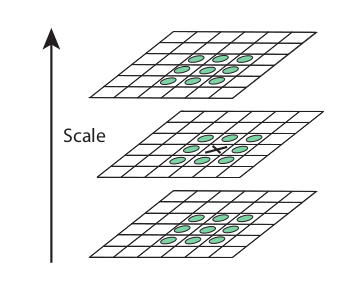
\includegraphics[width=0.4\linewidth]{images/DOG_maxmin_SIFT.png}
    \caption{The 3 samples per octave of difference of Gaussians used to compute the local minima/maxima.}
    \label{fig:DOG_maxmin_SIFT}
\end{figure}

\paragraph{Keypoint localization}
Given a set of keypoint candidates (found in the last setp by looking at the maxima and minima in the scale-space) the objective is to incorporate nearby data for location, scale and ratio of principal curvatures. This, as the author states, will help discard points of low contrast or poorly located along an edge. To do so, \cite{SIFT_Brown_Lowe} propose to fit a 3D quadratic function shifted to the keypoint candidate's position. It interpolates the location of the maximum, like so
\begin{equation} \label{eq:SIFT_quadratic_function}
    D(\mathbf{x})=D+\frac{\partial D^{T}}{\partial \mathbf{x}} \mathbf{x}+\frac{1}{2} \mathbf{x}^{\mathrm{T}} \frac{\partial^{2} D}{\partial \mathbf{x}^{2}} \mathbf{x}
\end{equation}
where $D$ and the derivatives are evaluated at the sample point and $x\left(\mathbf{x}, \mathbf{y}, \mathbf{\sigma}\right)^{\top}$ is the offset from said point. Taking the derivative and setting to 0 equation \ref{eq:SIFT_quadratic_function} yields the location at the extremum, $\hat{\mathbf{x}}$, like
\begin{equation} \label{eq:SIFT_quadratic_function_extremum}
    \hat{\mathbf{x}}=-\frac{\partial^{2} D^{-1}}{\partial \mathbf{x}^{2}} \quad \frac{\partial D}{\partial \mathbf{x}}
\end{equation}
From earlier equation it is easy to compute the derivative and the Hessian by making use of the difference of neighboring points. The author states that, if any dimension in $\mathbf{x}$ is larger that $0.5$, the extremum then actually lies closer to a different sample point. If that is the case, the sample point is changed and the interpolation in \ref{eq:SIFT_quadratic_function} is done for that larger point. Besides, all extrema with a value $|D(\hat{\mathbf{x}})| < 0.03$ are discarded.

The procedure shown allows to discard many keypoints that have low contrast, but edges still remain a problem. To tackle them, one needs to look at the principal curvature in a peak in the difference of Gaussians. Edges will have one large principal curvature and a smaller perpendicular one. The principal curvature can be computed form the Hessian at the location and scale fo the keypoint:
\begin{equation}
    \mathbf{H}=\left[\begin{array}{ll}
    D_{x x} & D_{x y} \\
    D_{x y} & D_{y y}
    \end{array}\right]
\end{equation}
The eigenvalues of $\mathbf{H}$ are proportional to the principal curvatures of $D$. The author mentions that the actual eigenvalues needn't be computed, since only their relation is of interest. Being $\alpha$ and $\beta$ the largest and smallest eigenvalues respectively, the trace and determinant of $\mathbf{H}$ will look like
\begin{equation}
    \begin{array}{c}
    \operatorname{Tr}(\mathbf{H})=D_{x x}+D_{y y}=\alpha+\beta \\
    \operatorname{Det}(\mathbf{H})=D_{x x} D_{y y}-\left(D_{x y}\right)^{2}=\alpha \beta
    \end{array}
\end{equation}
Being $r=\alpha/\beta$ the ratio between the eigenvalues, one can compute a relation between the trace and the determinant, like so
\begin{equation}
    \frac{\operatorname{Tr}(\mathbf{H})^{2}}{\operatorname{Det}(\mathbf{H})}=\frac{(\alpha+\beta)^{2}}{\alpha \beta}=\frac{(r \beta+\beta)^{2}}{r \beta^{2}}=\frac{(r+1)^{2}}{r}
\end{equation}
With this relation, under a given threshold\footnote{The author David Lowe uses $r=10$.} for $r$, one can discard a keypoint for being an edge just by computing the trace and the determinant. In other words, those keypoints below a certain value $\frac{(r+1)^{2}}{r}$ are discarded.

\paragraph{Orientation assignment} Having located good candidate keypoints the focus goes onto assigning a consistent orientation based on local properties. This is needed to have a keypoint invariant to image rotation. Every keypoint has a closest scale in the smoothed image $L$, from which the orientation $\theta(x,y)$and gradient magnitude $m(x,y)$ can be computed:
\begin{equation}
    \begin{array}{l}
    m(x, y)=\sqrt{(L(x+1, y)-L(x-1, y))^{2}+(L(x, y+1)-L(x, y-1))^{2}} \\
    \theta(x, y)=\tan ^{-1}((L(x, y+1)-L(x, y-1)) /(L(x+1, y)-L(x-1, y)))
    \end{array}
\end{equation}
The orientation is stored in a histogram with 36 bins (10º each), where each sample added to the histogram is weighted by its gradient magnitude and by a Gaussian-weighted circular window with a $\sigma$ 1.5 times that of the scale of the keypoint.

\paragraph{The local image descriptor}
Having a location, scale, and orientation to each keypoint one has a repeatable local 2D coordinate system in which to describe the local image region. There still remains, however, how to encode the information of said keypoint in a distinctive and invariant manner. \cite{SIFTlowe2004} presents a method in which gradient magnitudes and orientation are computed around the keypoint location in predefined window size of 16x16. They are weighted by a Gaussian window overlaid on top of the keypoint to avoid sudden changes in the descriptor with small changes in the position of the window, and to give less emphasis to gradients that are far from the center of the descriptor. In order to achieve orientation invariance the coordinates of the descriptor and the gradient orientations are rotated relative to the keypoint orientation. The image gradients in that window, then, are accumulated into orientation histograms in 4x4 regions. See figure \ref{fig:SIFT_keypoint_descriptor} for a visual example. 

To avoid boundary effects for the descriptor histogram trilinear interpolation is used. It will distribute the value of each gradient sample into adjacent histograms, and hence be more robust to abrupt changes for samples that shift smoothly from being within one histogram to another. In addition to this interpolation, each value in the histogram (a vector) is thresholded to 0.2 (that is, no value in the vector may be larger than 0.2), and the histogram vector is normalized to unit length. The former reduces the effect of nonlinear illumination changes (like camera saturation) and the latter to linear ones (like brightness variation).
\begin{figure}[htbp]
    \centering
    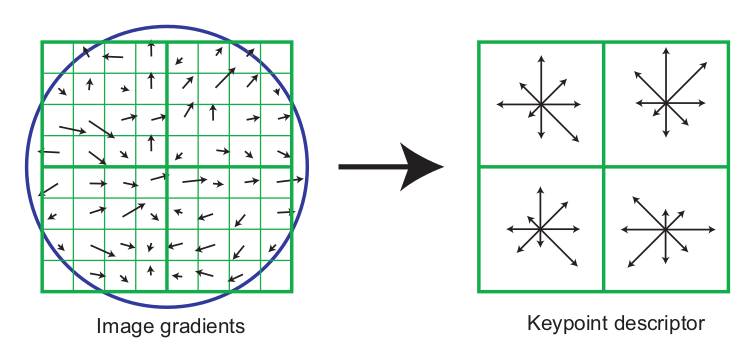
\includegraphics[width=0.8\linewidth]{images/SIFT_keypoint_descriptor.png}
    \caption{The creation of the keypoint: on the left, the image gradients and orientation are computed for each pixel in a window around the keypoint. Then a Gaussian window (blue circle overlaid on top of the window) is applied. The magnitude and orientation of these pixels are accumulated into the bins of a histogram  over 4x4 regions, as seen on the right. Each arrow represents the orientation and magnitude for that region. Note: the image shows a window of 8x8 and a keypoint descriptor with 2x2 regions. This is to make them visually simpler, but their actual sizes would be 16x16 and 4x4 respectively. Image extracted from \cite{SIFTlowe2004}.}
    \label{fig:SIFT_keypoint_descriptor}
\end{figure}

\paragraph{Object recognition using the SIFT algorithm} Object recognition is performed by matching the vector histogram of the keypoints in an image with those computed in a database of images. Many of the matches will be incorrect, as one may suppose, so \cite{SIFTlowe2004} states that at least clusters of 3 feature matches need to agree on the pose of the object.

Matching keypoint candidates are those with the nearest neighbor in the database of keypoints (from the database of images). The nearest neighbor is defined as the one with descriptor vector with the smallest Euclidean distance. However, a simple nearest neighbor is not enough for incorrect matchings coming from clutter of noise. \cite{SIFTlowe2004} discards using a global threshold since some descriptors are much more discriminative than others, and opts for comparing the distance of the closest neighbor to that of the second closest neighbor. A ratio of distance between the closest and second closest match is computed, and values beyond 0.8 are eliminated. The author asserts that this will eliminate 90\% of false matches while discarding only 5\% of correct matches\footnote{On the author's custom test suite.}. Rationale behind this is the following: false matches will tend to have many other false matches at a similar distance due to the high dimensionality of the feature space. The second closest match is thought of as an estimate of the density of false matches and ambiguity. 

After matchings are done, they need to be clustered. Some matchings will be incorrect, sure, but they can be filtered by considering their pose with respect to the others, and discard them if they differ too much from the consensus. \cite{SIFTlowe2004} uses the Hough transform in the pose space as the clustering technique since it is very robust to outliers (unlike RANSAC, which underperforms when outliers are above 50\%).




\subsection{Convolutional Neural Networks} \label{sec:world_neural_networks}

\subsubsection{Theoretical background}
% \subsection{The Convolutional Neural Network}
Arguably, Convolutional Neural Networks are one of the architectures inside the world of Artificial Intelligence that are most inspired by neuroscience. 
As stated by \cite{deep_learning_IGoodfellow} and \cite{hands_on_ML_Aurelien}, the history of convolutional networks begins with the collaborative research of neurophysiologists David H. Hubel and Torsten Wiesel. They widened the knowledge on the structure of the visual cortex experimenting with animals, showing that neurons in the visual cortex have a small \textit{local receptive field} that strongly reacts to imagery inside its corresponding region of the visual field of the animal. They also discovered that receptive fields of neurons overlap and construct layers, where the lower-level ones react to simple patterns (like lines with different orientations) and the ones connected on top of them react to more increasingly complex patterns. These studies culminated in what today are called Convolutional Neural Networks, which belong to the family of Deep Learning methods.

\paragraph{Computation with neurons in general: the Multi-Layer Perceptron}
A [simple] \textit{perceptron} is based on a \textit{linear threshold unit} (LTU). The LTU consists of one or more inputs with weights associated to each of them that converge to a weighted sum, and then applies a step function to it (commonly called activation function), as illustrated by Figure \ref{fig:simple_LTU}. The perceptron can be trained, and if increased in width (adding more LTUs) can solve some classification problems. Still, these systems are held back by important modelling limitations\footnote{Such as the XOR problem.} whose discussion is beyond the scope of this work.

\begin{figure}[H]
    \centering
    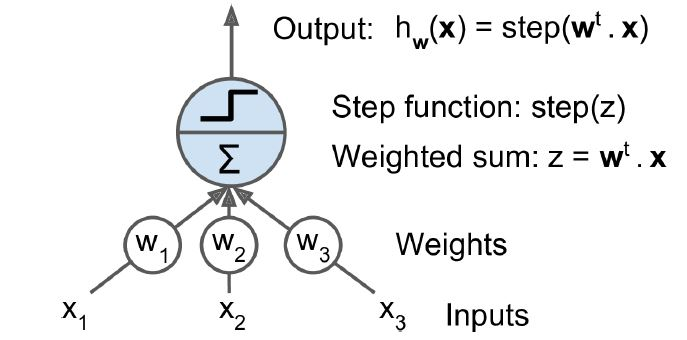
\includegraphics[width=0.7\linewidth]{images/simple_LTU.JPG}
    \caption{Perceptron of one linear threshold unit with three inputs. Figure extracted from \cite{hands_on_ML_Aurelien}.}
    \label{fig:simple_LTU}
\end{figure}

The Multi-Layer Perceptron (MLP), as the name suggests, is composed of several layers\footnote{Note that when the word "layers" in plural is used, the Artificial NN is called a Deep Neural Network (DNN).} of perceptrons with several LTUs stacked one upon the other and with nonlinear activation functions (every layer of LTUs includes one bias neuron), and lacks the data modelling limitations perceptrons suffer. Still, the main difficulty with MLPs is how to successfully train them.

Modern MLPs like the one in \ref{fig:MLP_with_RELU_and_Softmax} apply the \textit{backpropagation} training algorithm. For each training instance input to the MLP the final output is computed and compared against the true value it should have. This is the training error (that is, desired output minus actual output obtained). Then it is measured how the outputs of the intermediary neurons contributed to said training error and adjusts the weights of their connections. The way it is measured is by reversing directionality (from output to input of the MLP), hence the name of backpropagation. The ``adjustment'' on the weights of neurons is usually a Gradient Descent optimization algorithm (explained in the Appendix). This step is repeated until the training cannot be improved (convergence), or until a generalization maximum is reached.

A trainable MLP should also change the step function inside every neuron by a differentiable function\footnote{Which therefore has a gradient instead of a flat segment like the step function.} to allow use of the Gradient Descent as the training function inside the backpropagation algorithm. The step function was initially changed by the logistic function, $\sigma(z) = 1 / (1 + exp(-z))$, but the most common activation function is the Rectified Linear Unit (ReLU) $h_{w, b} = max(X \cdot w + b, 0)$\footnote{Where X is the input, w the weight and b the bias.}. It is also the type of activation function used in this work.

\begin{figure}[H]
    \centering
    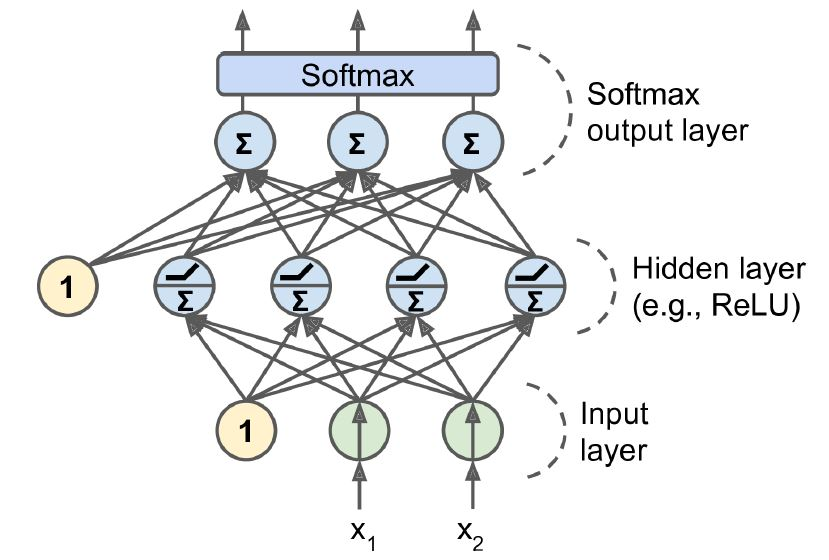
\includegraphics[width=0.7\linewidth]{images/MLP_with_RELU_and_Softmax.JPG}
    \caption{Multi-Layer Perceptron with Rectified Linear Units as activation and a Softmax layer as output. Figure extracted from \cite{hands_on_ML_Aurelien}.}
    \label{fig:MLP_with_RELU_and_Softmax}
\end{figure}

The MLP also requires a last layer for the output, which could be multiple (multi-class problem). This is accomplished with a \textit{softmax} layer, discussed in next subsection.

\paragraph{The softmax layer}
The best way to explain the softmax layer (that is, a layer that applies the softmax function) is by first introducing the linear regression, which is quite straightforward and represents the mapping from input to output as a linear combination of the form:

\begin{equation} \label{eqn:linear_regression}
    \hat{y} = \theta_0 + \theta_1 x_1 + \theta_2 x_2 + ... + \theta_n x_n,
\end{equation}
where $\hat{y}$ is the predicted value, $n$ is the number of input features, $x_i$ is the feature value (for example, if one wanted to predict the "level of success of a researcher", the input features could be the number of citations, the number of papers published and the number of conferences attended) and $\theta$ is the model parameter that multiplies each input feature (plus a bias term $ \theta_0 $). Equation \ref{eqn:linear_regression} can be easily vectorized as:

\begin{equation} \label{eqn:linear_regression_vectorized}
    \hat{y} = \theta^T \cdot \textbf{x},
\end{equation}
where $\theta^T$ is the parameters vector transposed (row vector) and \textbf{x} is the input feature vector ($x_0$ multiplied to $\theta_0$ is always 1).

The softmax function is a nonlinear counterpart to equation \ref{eqn:linear_regression_vectorized}, with the difference that it now supports several classes for every parameter vector. The output will therefore be a vector with as many values as classes, each one an estimation of the probability of the input value belonging to said class. The way this is done is by computing a score for each class, then computing its exponential and normalizing it. The score is calculated as:

\begin{equation} \label{eqn:softmax_score}
    s_{k}(\textbf{x}) = (\theta^{(k)})^T \cdot \textbf{x},
\end{equation}
where $s_k$ is the softmax score for every class $k$ and $\theta^(k)$ is the parameter vector for each class. Then:

\begin{equation} \label{eqn:softmax_function}
    \hat{p}_k = \frac{exp(s_{k}(\textbf{x}))}{\sum_{i=1}^{K} exp(s_{i}(\textbf{x}))}, 
\end{equation}
where $K$ is the total number of classes $k$, is the estimated output for each class.

Given the softmax function in \ref{eqn:softmax_function}, its classifier prediction takes the form of:

\begin{equation} \label{eqn:softmax_classifier_prediction}
    \hat{y} = \underset{k}{argmax} \; \; \hat{p}_k
\end{equation}

Equation \ref{eqn:softmax_classifier_prediction} thus returns the probability value of the most probable $k^{th}$ class. If, for example, $p_k$ is a 2 cell vector with values [0.89, 0.11], then class 1 (and not class 2) will be the most probable class for a given input vector, with a probability value of 0.89. So far, the functions behind the workings of the softmax layer have been exposed. But, how to determine the $\theta^{k}$ parameters introduced in equation \ref{eqn:softmax_score} to begin with? It is done by training the layer. How such thing can be done is explained in the following subsection.

\paragraph{Training of the softmax layer}
The key concept to understand the training of the softmax layer is the \textit{cost function}. To assess how well the model fits the training set, a performance measure must be used, and the most common one is the Mean Squared Error (MSE), described as: 

\begin{equation} \label{eqn:MSE_cost_function}
    MSE(\textbf{X}, \theta) = \frac{1}{m} \sum_{i=1}^{m} (\theta^T \cdot \textbf{x}^{i} - y^{i})^2
\end{equation}

In the end, the objective is to compare the prediction delivered by the training parameters and the true prediction for that input instance. It has to be noted that the MSE cost function has a closed-form solution, but that is not the case for other cost functions. Optimization algorithms like Gradient Descent are needed, and those will also need the gradient of the cost function to work.

With the concept of cost function explained, now the cost function for the softmax function is presented: the \textit{cross entropy cost function}\footnote{Yes, ``cost function'' was mentioned three times in just one sentence.} in equation \ref{eqn:cross_entropy_cost_function}. Note that $\Theta$ is the matrix of parameters:

\begin{equation} \label{eqn:cross_entropy_cost_function}
    J(\Theta) = -\frac{1}{m} \sum_{i=1}^{m} \sum_{k=1}^{K} y_k^{(i)}log\left(\hat{p}_k^{(i)}\right),
\end{equation}
where $K$ is the number of classes and $m$ is the number of training instances in the dataset. In fact, equation \ref{eqn:cross_entropy_cost_function} is the average cost function over the entire training set, hence the summation and the division by $m$.

Then, the \textit{gradient of the cross entropy} function for a class $k$ is defined as:
\begin{equation} \label{eqn:cross_entropy_gradient_function}
    \nabla_{\theta^{(k)}} J(\Theta) = \frac{1}{m} \sum_{i=1}^{m} \left(\hat{p}_k^{(i)} -  y_k^{(i)}\right).
\end{equation}
This equation  computes the gradient for every class $k$, so it should be evaluated as many times as classes exist. The result of using a Gradient Descent optimization algorithm will be a parameters matrix $\Theta$ with as many rows as input features and as many columns as classes.

Now that the basics of Deep Neural Networks have been seen, the focus shifts towards the special type of architecture that is used in this work: the Convolutional Neural Network.

\paragraph{The convolution operation and its implementation}
Let us suppose a 1D function $f(x)$ consisting on a series of delta functions along the axis, and another function $h(x)$ consisting on a Gauss continuous distribution. If $f$ is convolved\footnote{Denoted by an asterisk, although the symbol $\otimes$ is also used.} with $h$, which will be called $g(i)$, then:

\begin{equation} \label{eqn:1D_conv_cont}
    g(i) = (f \otimes h)(x) = \int_{-\infty}^{\infty} f(x) h(i-x) dx,
\end{equation}
as illustrated in figure \ref{fig:1d_convolution_example}. This particular example is inspired by a video series of the California Institute of Technology\footnote{https://www.youtube.com/watch?v=MQm6ZP1F6ms}.

\begin{figure}[H]
    \centering
    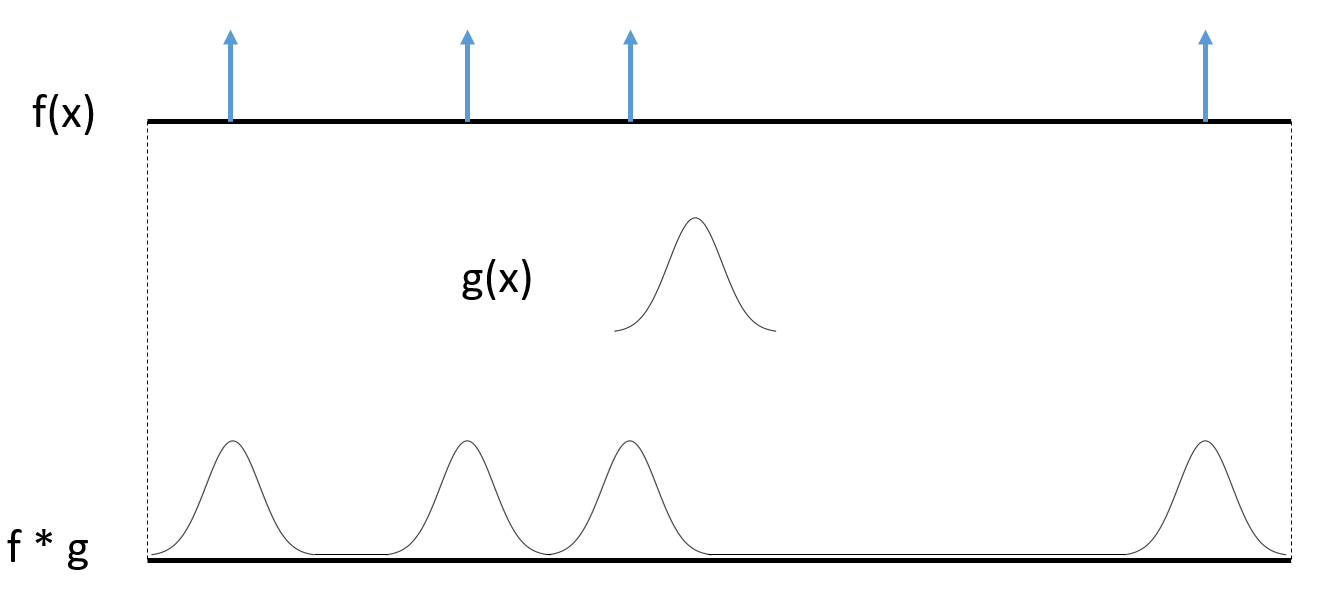
\includegraphics[width=0.9\linewidth]{images/1d_convolution_example.PNG}
    \caption{Delta functions distributed along an axis, $f(x)$, and a Gaussian distribution, $g(x)$. The convolution of $f$ with $g$ produces the function $f*g$, where the Gaussian is applied to every point in which $f(x)$ has the delta functions.}
    \label{fig:1d_convolution_example}
\end{figure}

A better way to represent the utility of the convolution is to exemplify it in 2 dimensions, which is the type CNNs usually deal with. Let us take the case of a finely pixelated image\footnote{Source: https://en.wikipedia.org/wiki/Convolution} like that in Figure \ref{fig:wiki_example_gaussian_blur} left. If the image, thought of as a 2D matrix, is convoluted with a Gaussian spreading function, the result is a blurred image like the one in \ref{fig:wiki_example_gaussian_blur} right. The mathematical rationale behind it is:

\begin{equation} \label{eqn:2D_conv_cont}
    g(i,j) = (f \otimes h)(x) = \int_{-\infty}^{\infty} \int_{-\infty}^{\infty} f(x,y) h(i-x,j-y) dxdy
\end{equation}

\begin{figure}[H]
    \centering
    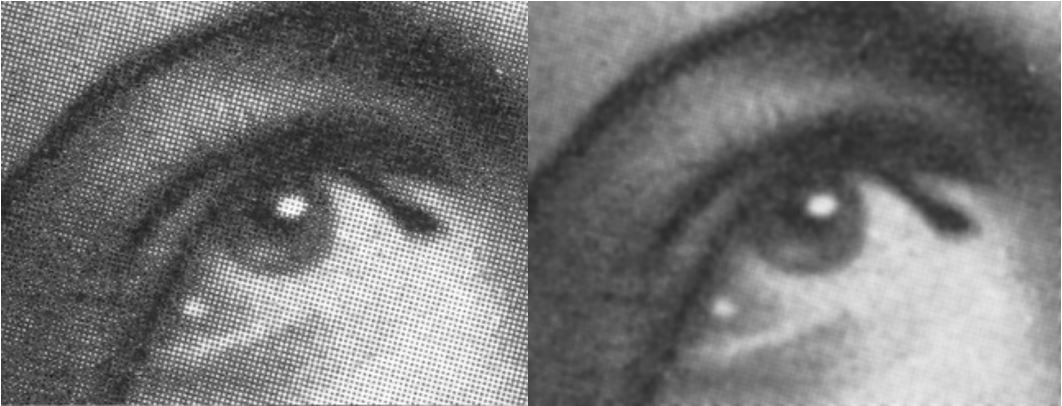
\includegraphics[width=\linewidth]{images/wiki_example_gaussian_blur.jpg}
    \caption{Finely pixelated image on the left, and after gaussian blur on the right.}
    \label{fig:wiki_example_gaussian_blur}
\end{figure}

But how does this translate into a computational scheme? There needs to be a discretization. For Eq. \ref{eqn:1D_conv_cont}, it is:

\begin{equation}
    g(i) = (f \otimes h)(i) = \sum_{x} f(x)*h(i-x),
\end{equation}
while for Eq. \ref{eqn:2D_conv_cont}:

\begin{equation} \label{eqn:2D_conv_disc}
    g(i,j) = (I \otimes K)(i,j) = \sum_{m} \sum_{n} I(m,n)K(i-m,j-n)
\end{equation}

In the ``convolutional network'' terminology, as stated in \cite{deep_learning_IGoodfellow}, $f(x)$ is considered the \textit{input} ($I$) and $h(x)$ the \textit{kernel} ($K$), and $g$, the output, is called \textit{feature map}. Thanks to the commutative property of the convolution, Eq. \ref{eqn:2D_conv_disc} can be written as: 

\begin{equation} \label{eqn:2D_conv_disc_2}
    g(i,j) = (K \otimes I)(i,j) = \sum_{m} \sum_{n} I(i-m,j-n)K(m,n)
\end{equation}
Eq. \ref{eqn:2D_conv_disc_2} is easier to implement because $K$ tends to have the same range of values. From Eq. \ref{eqn:2D_conv_disc_2}, it can be seen that as one index for the input increases, the index for the kernel decreases, and hence it can be said that said kernel is \textit{flipped}. Most CNN implementations avoid using the mathematical operation of convolution altogether (even though they still use the term\footnote{Which is also the case of this work.}) and use a very similar function called \textit{cross-correlation}, which does exactly the same as the convolution does, without flipping the kernel. It is described as:

\begin{equation} \label{eqn:2D_crosscorrel_disc}
    g(i,j) = (I \otimes K)(i,j) = \sum_{m} \sum_{n} I(i+m,j+n)K(m,n)
\end{equation}

The graphic representation of Eq. \ref{eqn:2D_crosscorrel_disc} is displayed in Figure \ref{fig:2D_conv_example}.

\begin{figure}[H]
    \centering
    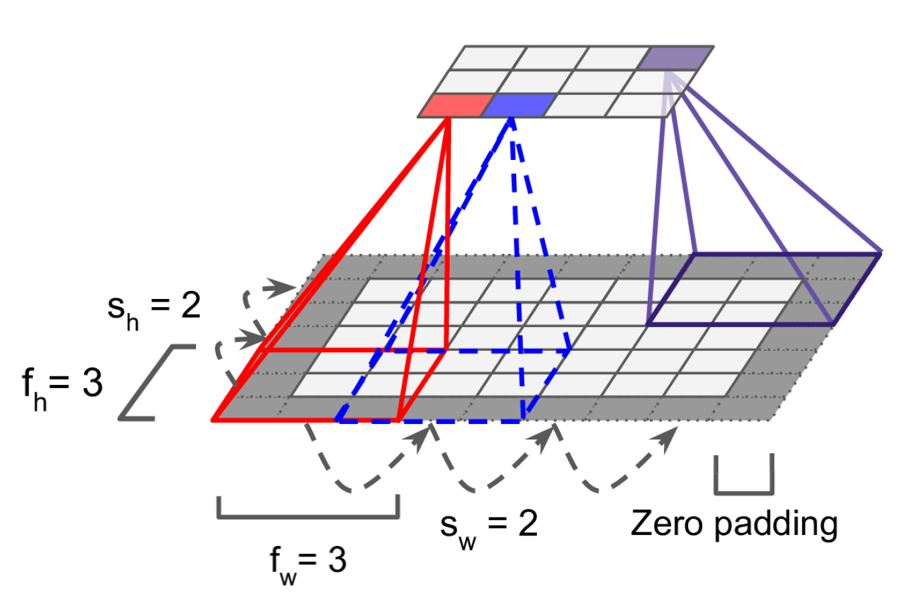
\includegraphics[width=0.7\linewidth]{images/2D_conv_example.JPG}
    \caption{Image from \cite{hands_on_ML_Aurelien} slightly edited. $f_h$ and $f_w$ stand for height and width of the receptive field, and can be understood as m and n of the cross-correlation function in \ref{eqn:2D_crosscorrel_disc}. It can be seen that the size of the output layer is smaller than the input layer. That is caused by the \textit{stride}, which is the distance from two consecutive receptive fields. Another important characteristic to point out is the existence of a zero-padding border surrounding the input. It is added to the input before the convolution to avoid the filter stepping out of bounds when it is being applied to the input. When stride = 1 the zero-padding also avoids shrinking the image, which allows an arbitrarily deep convolutional network.}
    \label{fig:2D_conv_example}
\end{figure}

\paragraph{A small remark on convolution kernels}
Convolution kernels, also called filters, hold the neurons' weights and can be represented as an image the size of the receptive field. Filters are designed to detect features in the input, and can increase in complexity as layers increase. Figure \ref{fig:filters_example}, for instance, shows two possible filters that result in two different feature maps. The one on the left will multiply by [almost] zero all things except for vertical lines, while the filter on the right will ignore everything except for horizontal lines. That is why the feature map of the left has vertical lines brighter (enhanced) and the rest is blurred out. A similar thing happens for the one on the right. The point of training a CNN is to find the most useful filters for the task, and combine them.

\begin{figure}[H]
    \centering
    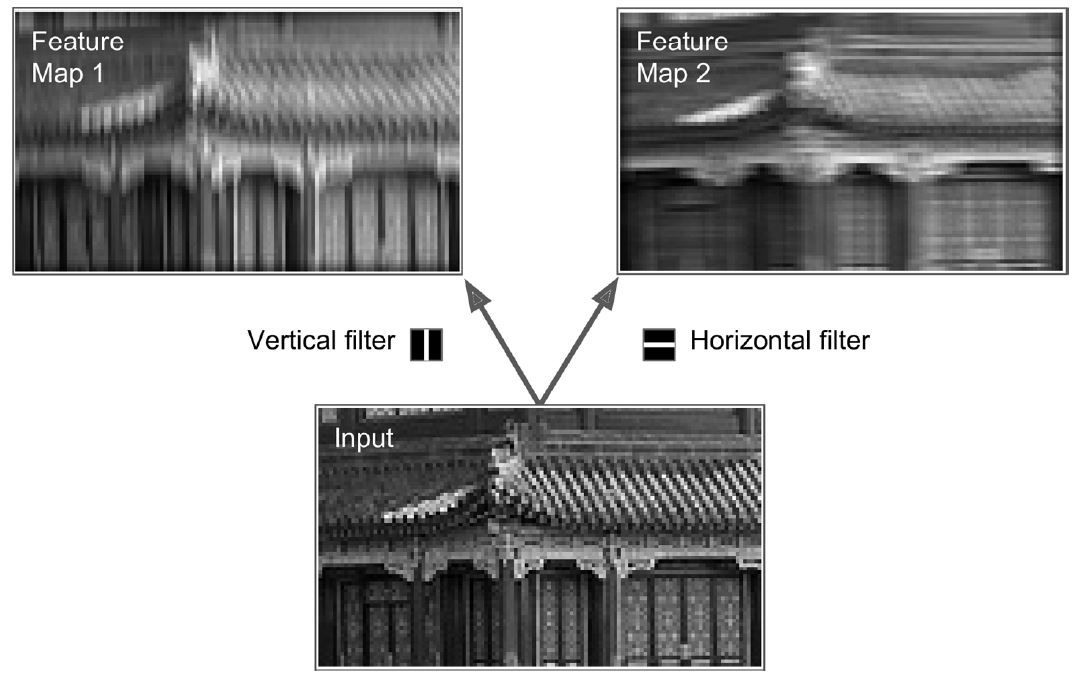
\includegraphics[width=0.8\linewidth]{images/filters_example.JPG}
    \caption{Image from \cite{hands_on_ML_Aurelien}. Two different filters to detect vertical and horizontal features on the input image will generate two feature maps.}
    \label{fig:filters_example}
\end{figure}


\paragraph{The feature maps}
The use of different filters on the same input will inevitably lead to as many outputs as filters applied. The way this is handled is by stacking said outputs one on top of another, creating a 3D matrix. To that end, the same procedure is applied again (as many times as convolutional layers the user desires). Image \ref{fig:conv_layers_and_feature_maps} visually explains this process.

\begin{figure}[H]
    \centering
    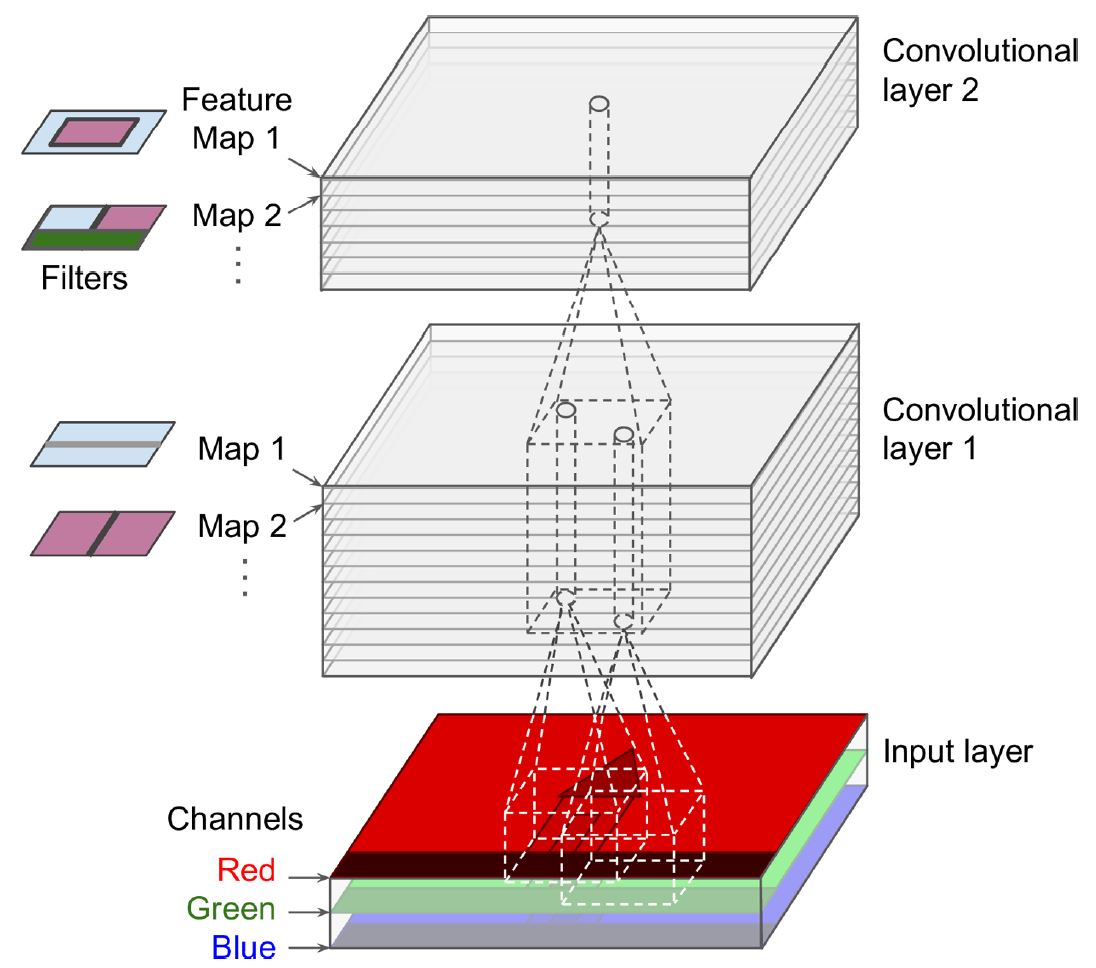
\includegraphics[width=0.8\linewidth]{images/conv_layers_and_feature_maps.JPG}
    \caption{Image from \cite{hands_on_ML_Aurelien}. Full color image represented by its three channels: Red, Green and Blue (RGB). A number of filters (kernels) are applied to the three channels, creating the same number of feature maps, which are stacked together. Higher-level convolution operations are applied to the previously stacked feature maps, with more complex filters to detect higher-level features.}
    \label{fig:conv_layers_and_feature_maps}
\end{figure}

\paragraph{More on training}
In previous subsections, the training method for both the softmax layer and backpropagation in NNs in general have been exposed. In this subsection, a brief explanation of the actual training method used on this work is delivered: the \textit{Root Mean Square back-Propagation} (RMSProp). The RMSProp algorithm was originally defined by Tijmen Tieleman and Geoffrey Hinton in 2012 for an educational video series for Coursera \cite{RMSProp_Coursera}, and greatly outperforms GD. 

RMSProp first calculates the accumulation of squares of gradients into vector $\textbf{s}$, but doing so for most recent iterations using an exponential weighted moving average (explained in the Appendix). Then, a very similar function to GD is used with the addition of an element-wise division: $\sqrt{\textbf{s} + \epsilon}$ \footnote{$\epsilon$ is a small arbitrary value to avoid division by zero.}. This scales down the jump in the gradient vector and allows to tackle one of the GD's main weaknesses: it does not rapidly go down the steepest slope, but rather move more gently, and eases the reach of a global minimum. In fact, this is called an \textit{adaptative learning rate}. Equations below show what has just been explained:

\begin{eqnarray} \label{eqn:GD_example_for_MSE}
    \textbf{s} \leftarrow \beta \textbf{s} + (1-\beta) \nabla_{\theta} J(\theta) \otimes \nabla_{\theta} J(\theta) \\
    \theta \leftarrow \theta - \eta \nabla_{\theta} \oslash \sqrt{\textbf{s} + \epsilon}
\end{eqnarray}

Apart from the RMSProp, other optimization algorithms are currently being used by the Machine Learning/Deep Learning community, such as Nesterov Accelerated Gradient, AdaGrad and Adam Optimization. Their explanation is, yet again, beyond the scope of this work.



\paragraph{The pooling layer}
The pooling layer is quite simple. As the name suggests, its objective is to make the input smaller by grouping its values. It is very useful to reduce computational cost (since further convolutional layers will have less parameters to tune, and the pooling layer itself has no weights) and memory consumption by extension. It will also give some tolerance to input image rotation or shift.

As with convolutional layers, the user needs to define a kernel size, stride, and a border padding. The pooling, which can be imagined as the action of taking one cell value from the matrix resulting of the projection of the pooling kernel on the input, can be accomplished by average or by maximum value. For example: in the first case, from a 2D matrix (which could have depth, therefore being 3D, but still the same applies) defined as [[2, 3], [4, 5]] the average result would be 3.5; in the second case, for that same example, the maximum would be 5. Nevertheless, figure \ref{fig:pooling_example} helps clarify this explanation.

\begin{figure}[H]
    \centering
    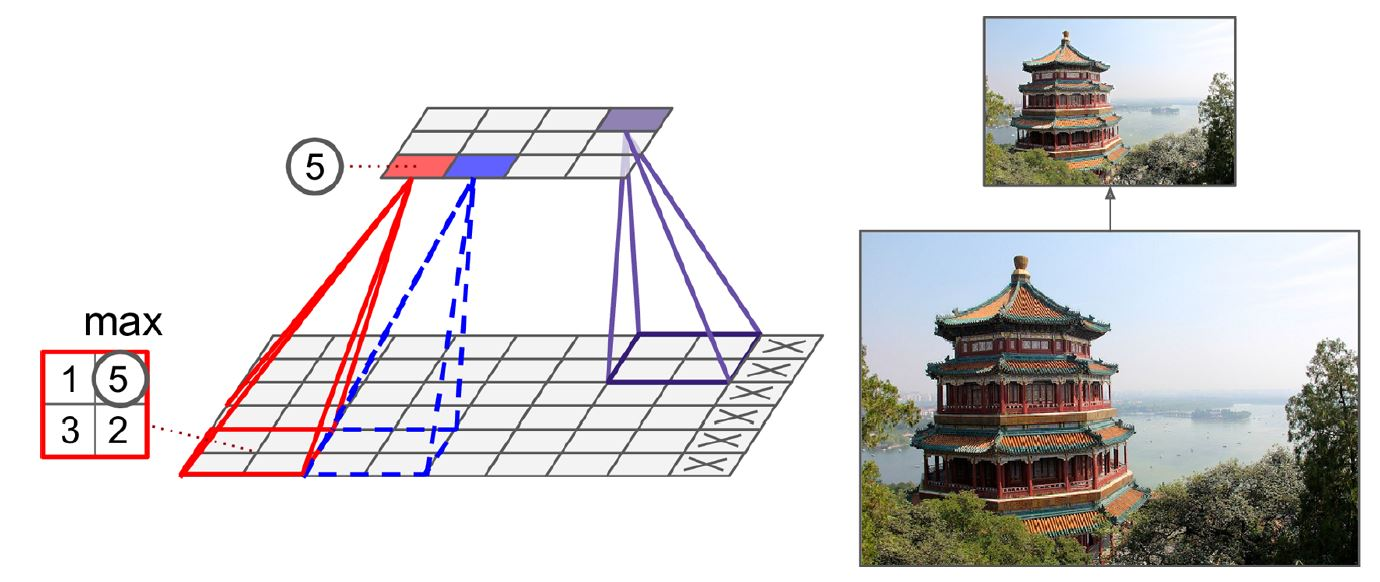
\includegraphics[width=0.8\linewidth]{images/pooling_example.JPG}
    \caption{Image from \cite{hands_on_ML_Aurelien}. Pooling layer in action. 2x2 kernel, stride of 2, no padding.}
    \label{fig:pooling_example}
\end{figure}

\subsubsection{Transfer learning}



\end{document}